\chapter{Reference Manuals for the \why Tools}
\label{chap:manpages}
%HEVEA\cutname{manpages.html}

This chapter details the usage of each of the command-line tools
provided by the \why environment. The main command is \texttt{why3};
it acts as an entry-point to all the features of \why. It is invoked
as such
\begin{verbatim}
why3 [general options...] <command> [specific options...]
\end{verbatim}

The following commands are available:
\begin{description}
\item[\texttt{bench}] produces benchmarks.
\item[\texttt{config}] manages the user's configuration,
  including the detection of installed provers.
\item[\texttt{doc}] produces HTML versions of \why source codes.
\item[\texttt{execute}] performs a symbolic execution of \whyml
  input files.
\item[\texttt{extract}] generates an OCaml program corresponding to
  \whyml input files.
\item[\texttt{ide}] provides a graphical interface to display goals
  and to run provers and transformations on them.
\item[\texttt{prove}] reads \why and \whyml input files and calls
  provers, on the command-line.
\item[\texttt{realize}] generates interactive proof skeletons for
  \why input files.
\item[\texttt{replay}] replays the proofs stored in a session,
  for regression test purposes.
\item[\texttt{session}] dumps various informations from a proof
  session, and possibly modifies the session.
\item[\texttt{wc}] gives some token statistics about \why and \whyml
  source codes.
\end{description}

All these commands are also available as standalone executable files,
if needed.

The commands accept a common subset of command-line options. In
particular, option \verb|--help| displays the usage and options.
\begin{description}
\item[\texttt{-L \textsl{<dir>}}]
  adds \texttt{\textsl{<dir>}} in the load path, to search for theories.
  \index{L@\verb+-L+|see{\texttt{-{}-library}}}
\item[\texttt{-{}-library \textsl{<dir>}}]
  is the same as \verb|-L|.
  \index{library@\verb+--library+}
\item[\texttt{-C \textsl{<file>}}]
  reads the configuration from the given file.
  \index{C@\verb+-C+|see{\texttt{-{}-config}}}
\item[\texttt{-{}-config \textsl{<file>}}]
  is the same as \verb|-C|.
  \index{config@\verb+--config+}
\item[\texttt{-{}-extra-config \textsl{<file>}}]
  reads additional configuration from the given file.
  \index{extra-config@\verb+--extra-config+}
\item[\texttt{-{}-list-debug-flags}]
  lists known debug flags.
  \index{list-debug-flags@\verb+--list-debug-flags+}
\item[\texttt{-{}-debug-all}]
  sets all debug flags (except flags which change the behavior).
  \index{debug-all@\verb+--debug-all+}
\item[\texttt{-{}-debug \textsl{<flag>}}]
  sets a specific debug flag.
  \index{debug@\verb+--debug+}
\item[\texttt{-{}-help}]
  displays the usage and the exact list of options for the given tool.
  \index{help@\verb+--help+}
\end{description}

\section{The \texttt{config} Command}
\label{sec:why3config}

\why must be configured to access external provers. Typically, this is done
by running the \texttt{config} command.
This must be done each time a new prover is installed.%
\index{config@\texttt{config}}%
\index{configuration file}

The provers that \why attempts to detect are described in
the readable configuration file \texttt{provers-detection-data.conf}
of the \why data directory (\eg
\texttt{/usr/local/share/why3}). Advanced users may try to modify this
file to add support for detection of other provers. (In that case,
please consider submitting a new prover configuration on the bug
tracking system.)

The result of provers detection is stored in the user's
configuration file (\verb+~/.why3.conf+ or, in the case of local
installation, \verb+why3.conf+ in \why sources top directory). This file
is also human-readable, and advanced users may modify it in order to
experiment with different ways of calling provers, \eg different
versions of the same prover, or with different options.

The \texttt{config} command also detects the plugins installed in the \why
plugins directory (\eg \texttt{/usr/local/lib/why3/plugins}). A
plugin must register itself as a parser, a transformation or a
printer, as explained in the corresponding section.
\index{plugin}

If the user's configuration file is already present,
\texttt{config} will only reset unset variables to default value,
but will not try to detect provers.
The option \verb|--detect-provers| should be used to force
\why to detect again the available
provers and to replace them in the configuration file. The option
\verb|--detect-plugins| will do the same for plugins.
\index{detect-provers@\verb+--detect-provers+}
\index{detect-plugins@\verb+--detect-plugins+}

If a supported prover is installed under a name
that is not automatically recognized by \texttt{why3config},
the option \verb|--add-prover| will add a specified binary
to the configuration. For example, an Alt-Ergo executable
\verb|/home/me/bin/alt-ergo-trunk| can be added as follows:
\begin{verbatim}
why3 config --add-prover alt-ergo /home/me/bin/alt-ergo-trunk
\end{verbatim}
As the first argument, one should put a prover
identification string. The list of known prover identifiers
can be obtained by the option \verb|--list-prover-ids|.
\index{add-prover@\verb+--add-prover+}
\index{list-prover-ids@\verb+--list-prover-ids+}

\section{The \texttt{prove} Command}
\label{sec:why3ref}

\why is primarily used to call provers on goals contained in an
input file. By default, such a file must be written either in \why language
(extension \texttt{.why}) or in \whyml language (extension \texttt{.mlw}).
However, a dynamically loaded
plugin can register a parser for some other format of logical problems,
\eg TPTP or SMT-LIB.
\index{prove@\texttt{prove}}

The \texttt{prove} command executes the following steps:
\begin{enumerate}
\item Parse the command line and report errors if needed.
\item Read the configuration file using the priority defined in
  Section~\ref{sec:whyconffile}.
\item Load the plugins mentioned in the configuration. It will not
  stop if some plugin fails to load.
\item Parse and typecheck the given files using the correct parser in order
  to obtain a set of \why theories for each file. It uses
  the filename extension or the \verb|--format| option to choose
  among the available parsers. \verb|why3 --list-formats| lists
  the registered parsers.
  \index{list-formats@\verb+--list-formats+}
  \whyml modules are turned into
  theories containing verification conditions as goals.
\item Extract the selected goals inside each of the selected theories
  into tasks. The goals and theories are selected using options
  \verb|-G/--goal| and \verb|-T/--theory|. Option
  \verb|-T/--theory| applies to the previous file appearing on the
  command line. Option \verb|-G/--goal| applies to the previous theory
  appearing on the command line. If no theories are selected in a file,
  then every theory is considered as selected. If no goals are selected
  in a theory, then every goal is considered as selected.
  \index{G@\verb+-G+|see{\texttt{-{}-goal}}}
  \index{goal@\verb+--goal+}
  \index{T@\verb+-T+|see{\texttt{-{}-theory}}}
  \index{theory@\verb+--theory+}
\item Apply the transformations requested
  with \verb|-a/--apply-transform| in their order of appearance on the
  command line. \verb|why3 --list-transforms| lists the known
  transformations; plugins can add more of them.
  \index{a@\verb+-a+|see{\texttt{-{}-apply-transform}}}
  \index{apply-transform@\verb+--apply-transform+}
  \index{list-transforms@\verb+--list-transforms+}
\item Apply the driver selected with the \verb|-D/--driver| option,
  or the driver of the prover selected with the \verb|-P/--prover|
  option. \verb|why3 --list-provers| lists the known provers, \ie the ones
  that appear in the configuration file.
  \index{D@\verb+-D+|see{\texttt{-{}-driver}}}
  \index{driver@\verb+--driver+}
  \index{P@\verb+-P+|see{\texttt{-{}-prover}}}
  \index{prover@\verb+--prover+}
  \index{list-provers@\verb+--list-provers+}
\item If option \verb|-P/--prover| is given, call the selected prover
  on each generated task and print the results. If option
  \verb|-D/--driver| is given, print each generated task using
  the format specified in the selected driver.
\end{enumerate}

%\texttt{why3} calls the provers sequentially, use \texttt{why3bench} if *)
%you want to call the provers concurrently.  *)

\subsection{Prover Results}
The provers can give the following output:
\begin{description}
\item[Valid] The goal is proved in the given context.
\item[Unknown] The prover has stopped its search.
\item[Timeout] The prover has reached the time limit.
\item[Failure] An error has occurred.
\item[Invalid] The prover knows the goal cannot be proved.
\end{description}
% \why can also be *)
% used to provide other informations : *)
% \begin{itemize} *)
% \item \texttt{print-namespace} print the namespace of the selected *)
%   theories *)
% \item TO BE COMPLETED *)
% \end{itemize} *)

%Option \verb|--bisect| changes the behavior of why3. With this
%option, \verb|-P/--prover| and \verb|-o/--output| must be given
%and a valid goal must be selected. The last step executed by why3 is
%replaced by computing a minimal set (in the great majority of the
%case) of declarations that still prove the goal. Currently it does not
%use any information provided by the prover; it calls the prover
%multiple times with reduced context. The minimal set of declarations is
%then written in the prover syntax into a file located in the directory
%given to the \verb|-o/--output| option.

\subsection{Additional Options}
\label{sec:proveoptions}

\begin{description}
\item[\texttt{-{}-get-ce}] activates the generation of a potential
counter-example when a proof does not succeed (experimental).
\item[\texttt{-{}-extra-expl-prefix \textsl{<s>}}] specifies
  \textsl{s} as an additional prefix for labels that denotes VC
  explanations. The option can be used several times to specify
  several prefixes.
\end{description}

\section{The \texttt{ide} Command}
\label{sec:ideref}

The basic usage of the GUI is described by the tutorial of
Section~\ref{sec:gui}. There are no specific command-line options,
apart from the common options detailed in introduction to this
chapter. However at least one anonymous argument must be specified on
the command line. More precisely, the first anonymous argument must be
the directory of the session. If the directory does not exist, it is
created. The other arguments should be existing files that are going
to be added to the session. For convenience,
if there is only one anonymous argument, it can be an existing file and
in this case the session directory is obtained by removing the extension
from the file name.

We describe the actions of the various menus and buttons of the
interface.
\index{ide@\texttt{ide}}

\subsection{Session}
\label{sec:idref:session}
\why stores in a session the way you achieve to prove goals that come
from a file (\texttt{.why}), from weakest-precondition (\texttt{.mlw}) or by other
means. A session stores which file you prove, by applying which
transformations, by using which prover. A proof attempt records the
complete name of a prover (name, version, optional attribute), the
time limit and memory limit given, and the result of the prover. The
result of the prover is the same as when you run the \texttt{prove} command. It
contains the time taken and the state of the proof:

\begin{description}
\item[Valid] The task is valid according to the prover. The
  goal is considered proved.
\item[Invalid] The task is invalid.
\item[Timeout] the prover exceeded the time limit.
\item[OufOfMemory] The prover exceeded the memory limit.
\item[Unknown] The prover cannot determine if the task
  is valid. Some additional information can be provided.
\item[Failure] The prover reported a failure.
\item[HighFailure] An error occurred while trying to call the
  prover, or the prover answer was not understood.
\end{description}

Additionally, a proof attempt can have the following attributes:

\begin{description}
\item[obsolete]\index{obsolete!proof attempt} The prover associated to
  that proof attempt has not been run on the current task, but on an
  earlier version of that task. You need to replay the proof
  attempt, \ie run the prover with the current task of the proof
  attempt, in order to update the answer of the prover and remove this
  attribute.
\item[archived]\index{archived!proof attempt} The proof attempt is not useful
  anymore; it is kept for history; no \why tools will select it by
  default. Section \ref{sec:uninstalledprovers} shows an example
  of this usage.
\end{description}

Generally, proof attempts are marked obsolete just after
the start of the user interface. Indeed, when you load a session in order to
modify it (not with \texttt{why3session info} for instance), \why
rebuilds the goals to prove by using the information provided in the
session. If you modify the original file (\texttt{.why}, \texttt{.mlw}) or if the
transformations have changed (new version of \why), \why will detect
that. Since the provers might answer differently on these new
proof obligations, the corresponding proof attempts are marked obsolete.

% non
% We say that a session is obsolete if new
% goals are made obsolete by this method during start-up.

% Claude: Alors la je ne vois pas pourquoi
% A session can
% be not obsolete even if it contains obsolete goals.

\subsection{Left toolbar actions}

\begin{description}
\item[Context] presents the context in which the other tools below will
  apply. If ``only unproved goals'' is selected, no action will ever
  be applied to an already proved goal.  If ``all goals'', then
  actions are performed even if the goal is already proved. The second
  choice allows to compare provers on the same goal.

\item[Strategies] section provides a set of actions that are
  performed on the selected goal(s):
  \begin{description}
  \item[Split] splits the current goal into subgoals if it is a
    conjunction of two or more goals. It corresponds to the
    \verb|split_goal_wp| transformation.
  \item[Inline] inlines the definitions in the conclusion of the goal.
    It corresponds to the \verb|introduce_premises| transformation
    follwoed by \verb|inline_goal|.
  \item[Auto level 1] is a strategy that first applies a few provers
    on the goal with a short time limit, then splits the goal and
    tries again on the subgoals
  \item[Auto level 2] is a strategy more elaborate than level 1, that
    attempts to apply a few transformations that are typically
    useful. It also tries the provers with a larger time limit.
  \end{description}
  A more detailed description of strategies is given in
  Section~\ref{sec:strategies}, as well as a description on how to
  design strategies of your own.

\item[Provers] provide a button for each detected prover. Clicking on such a
  button starts the corresponding prover on the selected goal(s).

% \item[Inline] replaces the head predicate symbol of the goal with its
%   definition. It corresponds to the
%   \verb|inline_goal| transformation.

\item[Tools] section provides a set of specific action that are
  typically performed on the selected goal(s). :
  \begin{description}
\item[Edit] starts an editor on the selected task.

  For automatic provers, this allows to see the file sent to the
  prover.

  For interactive provers, this also allows to add or modify the
  corresponding proof script. The modifications are saved, and can be
  retrieved later even if the goal was modified.

\item[Replay] replays all the obsolete proofs.

  If ``only unproved goals'' is selected, only formerly successful
  proofs are rerun. If ``all goals'', then all obsolete proofs are
  rerun, successful or not.

\item[Remove] removes a proof attempt or a transformation.

\item[Clean] removes any unsuccessful proof attempt for which there is
  another successful proof attempt for the same goal

\item[Interrupt] cancels all the proof attempts currently scheduled
  but not yet started.
\end{description}

\end{description}

\subsection{Menus}

\begin{description}
\item[Menu \textsf{File}]\emptyitem
\begin{description}
\item[Add File] adds a file in the GUI.
%\item[Detect provers] runs provers auto-detection
]\item[Preferences] opens a window for modifying preferred
  configuration parameters, see details below.
\item[Reload] reloads the input files from disk, and update the session state accordingly.
\item[Save session] saves current session state on disk. The policy to decide when to save the session is configurable, as described in the preferences below.
\item[Quit] exits the GUI.
\end{description}

\item[Menu \textsf{View}]\emptyitem
\begin{description}
\item[Expand All] expands all the rows of the tree view.
\item[Collapse proved goals] closes all the rows of the tree view
  that are proved.
% \item[Hide proved goals] completely hides the proved rows of the tree
%   view [EXPERIMENTAL]
\end{description}

\item[Menu \textsf{Tools}]
A copy of the tools already available in the left toolbar, plus:
\begin{description}
\item[Mark as obsolete] marks all the proof as
  obsolete.
  This allows to replay every proof.
\item[Non-splitting transformation] applies one of the available
  transformations, as listed in Section~\ref{sec:transformations}.
\item[Splitting transformation] is the same as above, but for
  splitting transformations, \ie those that can generate
  several sub-goals.
\end{description}

\item[Menu \textsf{Help}]
A very short online help, and some information about this software.
\end{description}

\subsection{Preferences Dialog}

The preferences dialog allows you to customize various settings. They
are grouped together under several tabs.

\begin{description}
\item[\textsf{General Settings} tab] allows one to set
  various general settings.
\begin{itemize}
\item the limits set on resource usages:
  \begin{itemize}
  \item the time limit given to provers, in seconds
  \item the memory given to provers, in megabytes
  \item the maximal number of simultaneous provers allowed to run in parallel
  \end{itemize}
  By default, modification of any of these settings has effect only
  for the current run of the GUI. A checkbox allows you to save these
  settings also for future sessions.
\item a few display settings:
  \begin{itemize}
  \item introduce premises: if selected, the goal of the task shown in
    top-right window is displayed after introduction of universally
    quantified variables and implications, \eg a goal of the form
    $\forall x: t. P \rightarrow Q$ is displayed as
    \[
    \begin{array}{l}
      x : t \\
      H : P \\
      \hline
      Q
    \end{array}
    \]
  \item show labels in formulas
  \item show source locations in formulas
  \item show time limit for each proof
  \end{itemize}
\item the policy for saving session:
  \begin{itemize}
  \item always save on exit (default): the current state of the proof session is saving on exit
  \item never save on exit: the current state of the session is never saved
    automatically, you must use menu \textsf{File/Save session}
  \item ask whether to save: on exit, a popup window asks whether you
    want to save or not.
  \end{itemize}
\end{itemize}
\item[\textsf{Editors} tab] allows one to customize the use
  of external editors for proof scripts.
\begin{itemize}
\item The default editor to use when the \textsf{Edit} button is
  pressed.
  \urldef{\urlprfgen}{\url}{http://proofgeneral.inf.ed.ac.uk/}
\item For each installed prover, a specific editor can be selected to
  override the default. Typically if you install the Coq prover, then
  the editor to use will be set to ``CoqIDE'' by default, and this
  dialog allows you to select the Emacs editor and its
 \ahref{\urlprfgen}{Proof General} mode instead%
 \begin{latexonly} (\urlprfgen)\end{latexonly}.
\end{itemize}
\item[\textsf{Provers} tab]
  allows to select which of the installed provers one wants to see
  as buttons in the left toolbar.
\item[\textsf{Uninstalled Provers} tab] presents all the
  decision previously taken for missing provers, as described in
  Section~\ref{sec:uninstalledprovers}. You can remove any recorded
  decision by clicking on it.
\end{description}

\subsection{Displaying Counterexamples}

When the selected prover finds (counterexample) model, it is possible to
display parts of this model in the terms of the original Why3 input.
Currently, this is supported for CVC4 prover version 1.5 and Z3.

To display the counterexample in Why3 IDE, the counterexample model generation
must be enabled in File -/> Preferences -/> get
counter-example.
After running the prover and clicking on the prover result in, the
counterexample can be displayed in the tab
Counter-example.
The counterexample is displayed with the original Why3 code in comments.
Counterexample values for Why3 source code elements at given line are
displayed in a comment at the line below.
An alternative way how to display a counterexample is to use the option
\texttt{-{}-get-ce} of the \texttt{prove} command.

Why3 source code elements that should be a part of counterexample must be
explicitly marked with \texttt{"model"} label. The following example shows a
Why3 theory with some terms annotated with the \texttt{model} label and the
generated counterexample in comments:

\begin{whycode}
theory T

  use import int.Int

  goal g_no_lab_ex : forall x:int. x >= 42 -> x + 3 <= 50

  goal g_lab_ex : forall x "model":int. ("model" x >= 42) ->
    ("model" "model_trace:x+3<=50" x + 3 <= 50)

  goal computation_ex : forall x1 "model" x2 "model" x3 "model" .
  (* x1 = 1; x2 = 1; x3 = 1 *)
  ("model" "model_trace: x1 + 1 = 2" x1 + 1 = 2) ->
  (*  x1 + 1 = 2 = true *)
  ("model" x2 + 1 = 2) ->
  (* (= (+ x2 1) 2) = true *)
  ("model" x3 + 1 = 2) ->
  (* (= (+ x3 1) 2) = true *)
  ("model" x1 + x2 + x3  = 5)
  (* (= (+ (+ x1 x2) x3) 5) = false *)
\end{whycode}

To display counterexample values in assertions the term being asserted must be
labeled with the label \texttt{"model\_vc"}. To display counterexample values
in postconditions, the term in the postcondition must be labeled with the
label \texttt{"model\_vc\_post"}.
The following example shows a counterexample of a function with postcondition:

\begin{whycode}
  let incr_ex ( x "model" : ref int ) (y "model" : ref int): unit
  (* x = -2; y = -2 *)
  ensures { !x = old !x + 2 + !y }
  =
  y := !y + 1;
  (* y = -1 *)
  x := !x + 1;
  (* x = -1 *)
  x := !x + 1
  (* x = 0 *)
\end{whycode}

It is also possible to rename counterexample elements using the lable
\texttt{"model\_trace:"}. The following example shows the use of renaming a
counterexample element in order to print the counterexample in infix notation
instead of default prefix notation:

\begin{whycode}
  goal g_lab_ex : forall x "model":int. ("model" x >= 42) ->
  (* x = 48; (<= 42 x) = true *)
    ("model" "model_trace:x+3<=50" x + 3 <= 50)
    (* x+3<=50 = false *)
\end{whycode}

Renaming counterexample elements is in particular useful when Why3 is used as
intermediate language and to show names of counterexample elements in the
source language instead of showing names of Why3 elements.
Note that if the counterexample element is of a record type, it is also
possible to rename names of the record fields by putting the label
\texttt{model\_trace:} to definitions of record fields. For example:

\begin{whycode}
  type r = {f "model_trace:.F" :int; g "model_trace:G" :bool}
\end{whycode}

When a prover is queried for a counterexample value of a term of an abstract
type=, an internal representation of the value is get. To get the concrete
representation, the term must be marked with the label
\texttt{"model\_projected"} and a projection function from the abstract type
to a concrete type must be defined, marked as a projection using the meta
\texttt{"model\_projection"}, and inlining of this function must be disabled
using the meta \texttt{"inline : no"}. The following example shows a
counterexample of an abstract value:

\begin{whycode}
  theory A

    use import int.Int

    type byte
    function to_rep byte : int
    predicate in_range (x : int) = -128 <= x <= 127
    axiom range_axiom : forall x:byte.
      in_range (to_rep x)
    meta "model_projection" function to_rep
    meta "inline : no" function to_rep

    goal abstr : forall x "model_projected" :byte. to_rep x >= 42 -> to_rep x
    + 3 <= 50
    (* x = 48 *)
\end{whycode}

More examples of using counterexample feature of Why3 can be found in the file
examples/tests/cvc4-models.mlw and examples/tests/cvc4-models.mlw.
More information how counterexamples in Why3 works can be found
in~\cite{hauzar16sefm}.

%
% how to use counterexamples - explain labels, projections, the option --get-ce of why3prove and the setting in why3ide
%
% problem with set logic and counterexamples
%
% which provers
%
% where it is displayed
%
% how to interpret the display
%
% example

\subsection{Additional Command-Line Options}

The \texttt{ide} command also accepts the following options described for the command \texttt{prove} in Section~\ref{sec:proveoptions}.
\begin{description}
\item[\texttt{-{}-extra-expl-prefix \textsl{<s>}}]
\end{description}


\section{The \texttt{bench} Command}

The \texttt{bench} command adds a scheduler on top of the \why
library. It is designed to compare various components
of automatic proofs: automatic provers, transformations, definitions
of a theory. For that purpose, it tries to prove predefined goals using
each component to compare. Various formats can be used as outputs:
\begin{description}
\item[\texttt{csv}] the simpler and more informative format; the results are
  represented in an array; the rows correspond to the
  compared components, the columns correspond to the result
  (Valid, Unknown, Timeout, Failure, Invalid) and the CPU time taken in seconds.
\item[\texttt{average}] it summarizes the number of the five different answers
  for each component. It also gives the average time taken.
\item[\texttt{timeline}] for each component, it gives the number of valid goals
  along the time (10 slices between 0 and the longest time a component
  takes to prove a goal)
\end{description}

The compared components can be defined in an \emph{rc-file};
\texttt{examples/misc/prgbench.rc} is an example of such a file. More
generally, a bench configuration file looks like
\begin{verbatim}
[probs "myprobs"]
   file = "examples/mygoal.why" #relatives to the rc file
   file = "examples/myprogram.mlw"
   theory = "myprogram.T"
   goal = "mygoal.T.G"

   transform = "split_goal" #applied in this order
   transform = "..."
   transform = "..."

[tools "mytools"]
   prover = cvc3
   prover = altergo
   #or only one
   driver = "..."
   command = "..."

   loadpath = "..." #added to the one in why3.conf
   loadpath = "..."

   timelimit = 30
   memlimit = 300

   use = "toto.T" #use the theory toto (allow to add metas)

   transform = "simplify_array" #only 1 to 1 transformation

[bench "mybench"]
   tools = "mytools"
   tools = ...
   probs = "myprobs"
   probs = ...
   timeline = "prgbench.time"
   average = "prgbench.avg"
   csv = "prgbench.csv"
\end{verbatim}

Such a file can define three families \texttt{tools}, \texttt{probs},
\texttt{bench}. A \texttt{tools} section defines a set of components to
compare. A \texttt{probs} section defines a set of goals on which to compare some
components. A \texttt{bench} section defines which components to
compare using which goals. It refers by name to some sections
\texttt{tools} and \texttt{probs} defined in the same file. The order
of the definitions is irrelevant. Notice that one can use
\texttt{loadpath} in a \texttt{tools} section to compare different
axiomatizations.

One can run all the bench given in one bench configuration file with
\begin{verbatim}
why3 bench -B path_to_my_bench.rc
\end{verbatim}

\section{The \texttt{replay} Command}
\label{sec:why3replayer}

The \texttt{replay} command is meant to execute the proofs
stored in a \why session file, as produced by the IDE. Its
main purpose is to play non-regression tests. For instance,
\texttt{examples/regtests.sh} is a script that runs regression tests on
all the examples.
\index{replay@\texttt{replay}}

The tool is invoked in a terminal or a script using
\begin{flushleft}\ttfamily
  why3 replay \textsl{[options] <project directory>}
\end{flushleft}
The session file \texttt{why3session.xml} stored in the given
directory is loaded and all the proofs it contains are rerun. Then,
all the differences between the information stored in the session file and
the new run are shown.

Nothing is shown when there is no change in the results, whether the
considered goal is proved or not. When all the proof
are done, a summary of what is proved or not is displayed using a
tree-shape pretty print, similar to the IDE tree view after doing
``Collapse proved goals''. In other words, when a goal, a theory, or a
file is fully proved, the subtree is not shown.

\paragraph{Obsolete proofs}

When some proof attempts stored in the session file are
obsolete\index{obsolete!proof attempt},
the replay is run anyway, as with the replay button in the IDE. Then, the session
file will be updated if both
\begin{itemize}
\item all the replayed proof attempts give the same result as what
  is stored in the session
\item every goals are proved.
\end{itemize}
In other cases, you can use the IDE to update the session, or use the
option \verb|--force| described below.

\paragraph{Exit code and options}

The exit code is 0 if no difference was detected, 1 if there
was. Other exit codes mean some failure in running the replay.

Options are:
\begin{description}
\item[\texttt{-s}] suppresses the output of the final tree view.
\item[\texttt{-q}] runs quietly (no progress info).
\item[\texttt{-{}-force}] enforces saving the session, if all proof
  attempts replayed correctly, even if some goals are not proved.
\item[\texttt{-{}-obsolete-only}] replays the proofs only if the session
  contains obsolete proof attempts.
\item[\texttt{-{}-smoke-detector \{none|top|deep\}}] tries to detect
  if the context is self-contradicting.
\item[\texttt{-{}-prover \textsl{<prover>}}] restricts the replay to the
  selected provers only.
\end{description}

\paragraph{Smoke detector}

The smoke detector tries to detect if the context is
self-contradicting and, thus, that anything can be proved in this
context. The smoke detector can't be run on an outdated session and does
not modify the session.  It has three possible configurations:
\begin{description}
\item[\texttt{none}] Do not run the smoke detector.
\item[\texttt{top}] The negation of each proved goal is sent with the
  same timeout to the prover that proved the original goal.
\begin{verbatim}
  Goal G : forall x:int. q x -> (p1 x \/ p2 x)
\end{verbatim}
  becomes
\begin{verbatim}
  Goal G : ~ (forall x:int. q x -> (p1 x \/ p2 x))
\end{verbatim}
  In other words, if the smoke detector is triggered, it means that the context
  of the goal \texttt{G} is self-contradicting.
\item[\texttt{deep}] This is the same technique as \texttt{top} but
  the negation is pushed under the universal quantification (without
  changing them) and under the implication. The previous example
  becomes
\begin{verbatim}
  Goal G : forall x:int. q x /\ ~ (p1 x \/ p2 x)
\end{verbatim}
  In other words, the premises of goal \texttt{G} are pushed in the
  context, so that if the smoke detector is triggered, it means that
  the context of the goal \texttt{G} and its premises are
  self-contradicting. It should be clear that detecting smoke in that
  case does not necessarily means that there is a mistake: for
  example, this could occur in the WP of a program with an unfeasible
  path.
\end{description}

At the end of the replay, the name of the goals that triggered the
smoke detector are printed:
\begin{verbatim}
  goal 'G', prover 'Alt-Ergo 0.93.1': Smoke detected!!!
\end{verbatim}
Moreover \texttt{Smoke detected} (exit code 1) is printed at the end
if the smoke detector has been triggered, or \texttt{No smoke
  detected} (exit code 0) otherwise.



\section{The \texttt{session} Command}
\label{sec:why3session}

The \texttt{session} command makes it possible to extract information from
proof sessions on the command line, or even modify them to some
extent. The invocation of this program is done under the form
\begin{verbatim}
why3 session <subcommand> [options] <session directories>
\end{verbatim}
The available subcommands are as follows:
\begin{description}
\item[\texttt{info}] prints informations and statistics about sessions.
\item[\texttt{latex}] outputs session contents in LaTeX format.
\item[\texttt{html}] outputs session contents in HTML format.
\item[\texttt{mod}] modifies some of the proofs, selected by a filter.
\item[\texttt{copy}] duplicates some of the proofs, selected by a filter.
\item[\texttt{copy-archive}] same as copy but also archives the
  original proofs\index{archived!proof attempt}.
\item[\texttt{rm}] removes some of the proofs, selected by a filter.
\end{description}

The first three commands do not modify the sessions, whereas the last
four modify them. Only the proof attempts recorded are modified. No
prover is called on the modified or created proof attempts, and
consequently the proof status is always marked as obsolete.

\subsection{Command \texttt{info}}

The command \texttt{why3 session info} reports various informations
about the session, depending on the following specific options.
\begin{description}
\item[\texttt{-{}-provers}] prints the provers that appear inside
  the session, one by line.
\item[\texttt{-{}-edited-files}] prints all the files that appear in
  the session as edited proofs.
\item[\texttt{-{}-stats}] prints various proofs statistics, as
  detailed below.
\item[\texttt{-{}-tree}] prints the structure of the session as a
  tree in ASCII, as detailed below.
\item[\texttt{-{}-print0}] separates the results of the options
  \verb|provers| and \verb|--edited-files| by the character number 0
  instead of end of line \verb|\n|. That allows you to safely use
  (even if the filename contains space or carriage return) the result
  with other commands. For example you can count the number of proof
  line in all the coq edited files in a session with:
\begin{verbatim}
why3 session info --edited-files vstte12_bfs --print0 | xargs -0 coqwc
\end{verbatim}
  or you can add all the edited files in your favorite repository
  with:
\begin{verbatim}
why3 session info --edited-files --print0 vstte12_bfs.mlw | \
    xargs -0 git add
\end{verbatim}

\end{description}

\paragraph{Session Tree}

The hierarchical structure of the session is printed as a tree in
ASCII. The files, theories, goals are marked with a question mark
\verb|?|, if they are not verified. A proof is usually said to be
verified if the proof result is \verb|valid| and the proof is not
obsolete.
However here specially we separate these two properties. On
the one hand if the proof suffers from an internal failure we mark it
with an exclamation mark \verb|!|, otherwise if it is not valid we
mark it with a question mark \verb|?|, finally if it is valid we add
nothing. On the other hand if the proof is obsolete we mark it with an
\verb|O| and if it is archived we mark it with an \verb|A|.

For example, here are the session tree produced on the ``hello
proof'' example of Section~\ref{chap:starting}.
{\scriptsize
\begin{verbatim}
hello_proof---../hello_proof.why?---HelloProof?-+-G3-+-Simplify (1.5.4)?
                                                |    `-Alt-Ergo (0.94)
                                                |-G2?-+-split_goal?-+-G2.2-+-Simplify (1.5.4)
                                                |     |             |      `-Alt-Ergo (0.94)
                                                |     |             `-G2.1?-+-Coq (8.3pl4)?
                                                |     |                     |-Simplify (1.5.4)?
                                                |     |                     `-Alt-Ergo (0.94)?
                                                |     |-Simplify (1.5.4)?
                                                |     `-Alt-Ergo (0.94)?
                                                `-G1---Simplify (1.5.4)
\end{verbatim}
}

\paragraph{Session Statistics}

The proof statistics given by option \verb|--stats| are as follows:
\begin{itemize}
\item Number of goals: give both the total number of goals, and the
  number of those that are proved (possibly after a transformation).
\item Goals not proved: list of goals of the session which are not
  proved by any prover, even after a transformation.
\item Goals proved by only one prover: the goals for which there is only
  one successful proof. For each of these, the prover which was
  successful is printed. This also includes the sub-goals generated by
  transformations.
\item Statistics per prover: for each of the prover used in the
  session, the number of proved goals is given. This also includes the
  sub-goals generated by transformations. The respective minimum,
  maximum and average time and on average running time is
  shown. Beware that these time data are computed on the
  goals \emph{where the prover was successful}.
\end{itemize}

For example, here are the session statistics produced on the ``hello
proof'' example of Section~\ref{chap:starting}.
{\footnotesize
\begin{verbatim}
== Number of goals ==
  total: 5  proved: 3

== Goals not proved ==
  +-- file ../hello_proof.why
    +-- theory HelloProof
      +-- goal G2
        +-- transformation split_goal
          +-- goal G2.1

== Goals proved by only one prover ==
  +-- file ../hello_proof.why
    +-- theory HelloProof
      +-- goal G1: Simplify (1.5.4) (0.00)
      +-- goal G3: Alt-Ergo (0.94) (0.00)

== Statistics per prover: number of proofs, time (minimum/maximum/average) in seconds ==
  Alt-Ergo (0.94)      :   2   0.00   0.00   0.00
  Simplify (1.5.4)     :   2   0.00   0.00   0.00

\end{verbatim}
}

\subsection{Command \texttt{latex}}

Command \texttt{latex} produces a summary of the replay under the form
of a tabular environment in LaTeX, one tabular for each theory, one
per file.

The specific options are
\begin{description}
\item[\texttt{-style \textsl{<n>}}] sets output style (1 or 2, default 1)
  Option \texttt{-style 2} produces an alternate version of LaTeX
  output, with a different layout of the tables.
\item[\texttt{-o \textsl{<dir>}}] indicates where
  to produce LaTeX files (default: the session directory).
\item[\texttt{-longtable}] uses the `longtable' environment instead of
  `tabular'.
\item[\texttt{-e \textsl{<elem>}}] produces a table for the given element, which is
  either a file, a theory or a root goal. The element must be specified
  using its path in dot notation, \eg \verb|file.theory.goal|. The
  file produced is named accordingly,
  \eg \verb|file.theory.goal.tex|.  This option can be given several
  times to produce several tables in one run. When this option is
  given at least once, the default behavior that is to produce one
  table per theory is disabled.
\end{description}

\paragraph{Customizing LaTeX output}

The generated LaTeX files contain some macros that must be defined
externally.  Various definitions can be given to them to customize the
output.
\begin{description}
\item[\texttt{\bs{}provername}] macro with one parameter, a prover name
\item[\texttt{\bs{}valid}] macro with one parameter, used where the corresponding prover answers that the goal is valid. The parameter is the time in seconds.
\item[\texttt{\bs{}noresult}] macro without parameter, used where no result
  exists for the corresponding prover
\item[\texttt{\bs{}timeout}] macro without parameter, used where the corresponding prover reached the time limit
\item[\texttt{\bs{}explanation}] macro with one parameter, the goal name or its explanation
\end{description}

\begin{figure}[t]
\begin{center}
\lstinputlisting[basicstyle={\ttfamily\small}]{./replayer_macros.tex}
\end{center}
\caption{Sample macros for the LaTeX command}
\label{fig:custom-latex}
\end{figure}

\begin{figure}[t]
\begin{center}
%HEVEA\begin{toimage}
\begin{tabular}{| l |c |c |c |c |c |}
\hline \multicolumn{2}{|c|}{Proof obligations } & \provername{Alt-Ergo 0.93} & \provername{Coq 8.2pl1} & \provername{Simplify 1.5.4} \\ 
\hline 
\explanation{G1} & \explanation{ }& \noresult& \noresult& \valid{0.01} \\ 
\hline 
\explanation{G2} & \explanation{ }& \noresult& \noresult& \unknown \\ 
\cline{2-5} 
\explanation{ }& \explanation{ }\explanation{G2.1} & \unknown & \unknown & \unknown \\ 
\cline{2-5} 
\explanation{ }& \explanation{ }\explanation{G2.2} & \valid{0.02} & \noresult& \valid{0.01} \\ 
\hline 
\explanation{G3} & \explanation{ }& \valid{0.02} & \noresult& \unknown \\ 
\hline \end{tabular}

%HEVEA\end{toimage}
%HEVEA\imageflush
\end{center}
\caption{LaTeX table produced for the HelloProof example (style 1)}
\label{fig:latex}
\end{figure}

\begin{figure}[t]
\begin{center}
%HEVEA\begin{toimage}
\begin{tabular}{| l |c |c |c |c |c |}
\hline Proof obligations & \provername{Alt-Ergo (0.94)} & \provername{Coq (8.3pl4)} & \provername{Simplify (1.5.4)} \\ 
\hline 
\explanation{G1} & \noresult& \noresult& \valid{0.00} \\ 
\hline 
\explanation{G2} & \unknown{0.00} & \noresult& \unknown{0.00} \\ 
\cline{2-4} 
\quad\transformation{split\_goal} & \multicolumn{3}{|c|}{}\\ 
\cline{2-4} 
\quad\subgoal{G2.1}{1} & \unknown{0.00} & \unknown{0.49} & \unknown{0.00} \\ 
\cline{2-4} 
\quad\subgoal{G2.2}{2} & \valid{0.00} & \noresult& \valid{0.00} \\ 
\hline 
\explanation{G3} & \valid{0.00} & \noresult& \unknown{0.00} \\ 
\hline \end{tabular}

%HEVEA\end{toimage}
%HEVEA\imageflush
\end{center}
\caption{LaTeX table produced for the HelloProof example (style 2)}
\label{fig:latexstyle2}
\end{figure}

Figure~\ref{fig:custom-latex} suggests some definitions for these
macros, while Figures~\ref{fig:latex} and~\ref{fig:latexstyle2} show
the tables obtained from the HelloProof example of
Section~\ref{chap:starting}, respectively with style 1 and 2.

\subsection{Command \texttt{html}}

This command produces a summary of the proof session in HTML syntax.
There are two styles of output: `table' and `simpletree'. The default is
`table'.

The file generated is named \texttt{why3session.html} and is written
in the session directory by default (see option \texttt{-o} to
override this default).

\begin{figure}[t]
%BEGIN LATEX
\begin{center}
\fbox{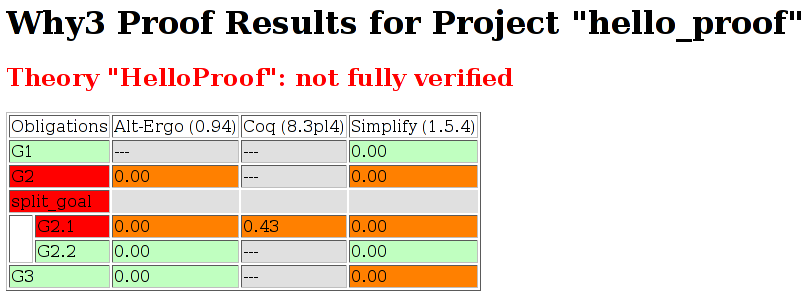
\includegraphics[width=0.9\textwidth]{hello_proof.png}}
\end{center}
%END LATEX
\begin{htmlonly}
\begin{rawhtml}
<h1>Why3 Proof Results for Project "hello_proof"</h1>
<h2><font color="#FF0000">Theory "HelloProof": not fully verified</font></h2>
<table border="1"><tr><td colspan="2">Obligations</td><td text-rotation="90">Alt-Ergo (0.94)</td><td text-rotation="90">Coq (8.3pl4)</td><td text-rotation="90">Simplify (1.5.4)</td></td></tr>
<td bgcolor="#C0FFC0" colspan="2">G1</td><td bgcolor="#E0E0E0">---</td><td bgcolor="#E0E0E0">---</td><td bgcolor="#C0FFC0">0.00</td></tr>
<td bgcolor="#FF0000" colspan="2">G2</td><td bgcolor="#FF8000">0.00</td><td bgcolor="#E0E0E0">---</td><td bgcolor="#FF8000">0.00</td></tr>
<tr><td bgcolor="#FF0000" colspan="2">split_goal</td><td bgcolor="#E0E0E0"></td><td bgcolor="#E0E0E0"></td><td bgcolor="#E0E0E0"></td></tr>
<td rowspan="2">&nbsp;&nbsp;</td><td bgcolor="#FF0000" colspan="1">1.</td><td bgcolor="#FF8000">0.00</td><td bgcolor="#FF8000">0.43</td><td bgcolor="#FF8000">0.00</td></tr>
<tr><td bgcolor="#C0FFC0" colspan="1">2.</td><td bgcolor="#C0FFC0">0.00</td><td bgcolor="#E0E0E0">---</td><td bgcolor="#C0FFC0">0.00</td></tr>
<td bgcolor="#C0FFC0" colspan="2">G3</td><td bgcolor="#C0FFC0">0.00</td><td bgcolor="#E0E0E0">---</td><td bgcolor="#FF8000">0.00</td></tr>
</table>
\end{rawhtml}
\end{htmlonly}
\caption{HTML table produced for the HelloProof example}
\label{fig:html}
\end{figure}

The style `table' outputs the contents of the session as a table,
similar to the LaTeX output above. Figure~\ref{fig:html} is the HTML
table produced for the `HelloProof' example, as typically shown in a
Web browser. The gray cells filled with \texttt{---} just mean that
the prover was not run on the corresponding goal. Green background
means the result was ``Valid'', other cases are in orange
background. The red background for a goal means that the goal was not
proved.

The style `simpletree' displays the contents of the session under the
form of tree, similar to the tree view in the IDE. It uses only basic
HTML tags such as \verb|<ul>| and \verb|<li>|.

Specific options for this command are as follows.
\begin{description}
\item[\texttt{-{}-style \textsl{<style>}}] sets the style to use, among
  \texttt{simpletree} and \texttt{table}; defaults to
  \texttt{table}.

\item[\texttt{-o \textsl{<dir>}}] sets the directory where to output
  the produced files (`\texttt{-}' for stdout). The default is to output
  in the same directory as the session itself.

\item[\texttt{-{}-context}] adds context around the generated code in
  order to allow direct visualization (header, css, ...). It also adds
  in the output directory all the needed external files. It can't be set with
  stdout output.

\item[\texttt{-{}-add\_pp \textsl{<suffix>} \textsl{<cmd>} \textsl{<out\_suffix>}}] sets a specific
  pretty-printer for files with the given suffix. Produced files use
  \texttt{\textsl{<out\_suffix>}} as suffix. \texttt{\textsl{<cmd>}} must contain
  `\texttt{\%i}' which will be replaced by the input file and
  `\texttt{\%o}' which will be replaced by the output file.

\item[\texttt{-{}-coqdoc}] uses the \verb|coqdoc| command to display Coq proof
  scripts. This is equivalent to \texttt{-{}-add\_pp .v "coqdoc
    -{}-no-index -{}-html -o \%o \%i" .html}

\end{description}

\subsection{Commands modifying the proof attempts}

The commands \texttt{mod}, \texttt{copy}, \texttt{copy-archive},
and \texttt{rm}, share the same set of options for selecting the proof
attempts to work on:
\begin{description}
\item[\texttt{-{}-filter-prover \textsl{<prover>}}] selects only the proof attempt with
  the given prover. This option can be specified multiple times in order
  to select all the proofs that corresponds to any of the given
  provers.
\item[\texttt{-{}-filter-verified yes}] selects only
  the proofs that are valid and not obsolete, while option
  \verb|--filter-verified no| selects the ones that are not verified.
  \verb|--filter-verified all|, the default, does not perform such a selection.
\item[\texttt{-{}-filter-verified-goal yes}] restricts the selection
  to the proofs of verified goals (that does not mean that the proof is
  verified). Same for the other cases \verb|no| and \verb|all|.
\item[\texttt{-{}-filter-archived yes}] restricts the selection
  to the proofs that are archived.
  Same for the other cases \verb|no|
  and \verb|all| except the default is \verb|no|.
\end{description}

\noindent
The commands \texttt{mod}, \texttt{copy}, and \texttt{copy-archive},
share the same set of options to specify the modification. The
command \texttt{mod} modifies directly the proof attempt,
\texttt{copy} copies the proof attempt before doing the modification,
\texttt{copy-archive} marks the original proof attempt as
archived.
The options are:
\begin{description}
\item[\texttt{-{}-set-obsolete}] marks the selected proofs as
  obsolete.
\item[\texttt{-{}-set-archived}] marks the selected proofs as archived.
\item[\texttt{-{}-unset-archived}] removes the archived attribute
  from the selected proofs.
\item[\texttt{-{}-to-prover \textsl{<prover>}}] modifies the prover, for example
  \texttt{-{}-to-prover Alt-Ergo,0.94}. A conflict arises if a proof
  with this prover already exists. In this case, you can choose between four
  behaviors:
\begin{itemize}
\item replace the proof (\verb|-f|, \verb|--force|);
\item do not replace the proof (\verb|-n|, \verb|--never|);
\item replace the proof unless it is verified (valid and not
  obsolete) (\verb|-c|, \verb|--conservative|); this is the default;
\item ask the user each time the case arises (\verb|-i|, \verb|--interactive|).
\end{itemize}
\end{description}

The command \texttt{rm} removes the selected proof
attempts. The options \verb|--interactive|, \verb|--force|, and
\verb|--conservative|, can also be used to respectively ask before
each suppression, suppress all the selected proofs (default), and remove
only the proofs that are not verified. The macro option \verb|--clean|
corresponds to \verb|--filter-verified-goal --conservative| and
removes the proof attempts that are not verified but which correspond
to verified goals.

The commands of this section do not accept by default to modify an
obsolete session (as defined in \ref{sec:idref:session}). You need to
add the option \verb|-F| to force this behavior.


% pour l'instant on ne documente pas parce que commenté dans le code
% \todo{A adapter en fonction de la decision sur l'upgrade de prover}

% If you just want to update one session with updated provers you can
% use \verb|--convert-unknown| instead of the option \verb|--to-prover|.
% \begin{verbatim}
% why3session copy  --convert-unknown
% \end{verbatim}
% For each proof attempt associated to an unknown prover (a prover not in
% \verb|.why3.conf|) and not archived, it will try to find a known prover
% with the same name. If it finds one, the proof attempt is copied to this
% prover and the old proof is set to archived. The corresponding edited
% files, if any, are copied and regenerated for the new prover An archived
% proof is not replayed by why3replayer.



\section{The \texttt{doc} Command}
\label{sec:why3doc}

This tool can produce HTML pages from \why source code.
\why code for theories or modules is output in
preformatted HTML code. Comments are interpreted in three different ways.
\begin{itemize}
\item Comments starting with at least three stars are completed
  ignored.
\item Comments starting with two stars are interpreted as textual
  documentation. Special constructs are interpreted as described
  below. When the previous line is not empty, the comment is indented to
  the right, so as to be displayed as a description of that line.
\item Comments starting with one star only are interpreted as code
  comments, and are typeset as the code
\end{itemize}

Additionally, all the \why identifiers are typeset with links so that
one can navigate through the HTML documentation, going from some
identifier use to its definition.

\paragraph{Options}

\begin{description}
\item[\texttt{-o \textsl{<dir>}}] defines the directory where to
  output the HTML files.
\item[\texttt{-{}-output \textsl{<dir>}}] is the same as \verb|-o|.
\item[\texttt{-{}-index}] generates an index file \texttt{index.html}.
  This is the default behavior if more than one file
  is passed on the command line.
\item[\texttt{-{}-no-index}] prevents the generation of an index file.
\item[\texttt{-{}-title \textsl{<title>}}] sets title of the
  index page.
\item[\texttt{-{}-stdlib-url \textsl{<url>}}] sets a URL for files
  found in load path, so that links to definitions can be added.
\end{description}

\paragraph{Typesetting textual comments}

Some constructs are interpreted:
\begin{itemize}
\item \texttt{\{\textsl{c text}\}} interprets character \textsl{c} as
  some typesetting command:
  \begin{description}
  \item[1-6] a heading of level 1 to 6 respectively
  \item[h] raw HTML
  \end{description}
\item \texttt{[\textsl{code}]} is a code escape: the text
  \textsl{code} is typeset as \why code.
\end{itemize}

A CSS file \verb|style.css| suitable for rendering is generated in the
same directory as output files. This CSS style can be modified manually,
since regenerating the HTML documentation will not overwrite an existing
\verb|style.css| file.

\section{The \texttt{execute} Command}
\label{sec:why3execute}

\why can symbolically execute programs written using the \whyml language
(extension \texttt{.mlw}). See also Section~\ref{sec:execute}.
\index{execute@\texttt{execute}}

\section{The \texttt{extract} Command}
\label{sec:why3extract}

\why can extract programs written using the \whyml language
(extension \texttt{.mlw}) to OCaml. See also Section~\ref{sec:extract}.
\index{extract@\texttt{extract}}

\section{The \texttt{realize} Command}
\label{sec:why3realize}

\why can produce skeleton files for proof assistants that, once filled,
realize the given theories. See also Section~\ref{sec:realizations}.
\index{realize@\texttt{realize}}

\section{The \texttt{wc} Command}
\label{sec:why3wc}

\why can give some token statistics about \why and \whyml source codes.
\index{wc@\texttt{wc}}

%%% Local Variables:
%%% mode: latex
%%% TeX-PDF-mode: t
%%% TeX-master: "manual"
%%% End:
